\documentclass[conf]{new-aiaa}
%\documentclass[journal]{new-aiaa} for journal papers
\usepackage[utf8]{inputenc}
\usepackage{listings}
\usepackage{graphicx}
\usepackage{amsmath}
\usepackage[version=4]{mhchem}
\usepackage{siunitx}
\usepackage{longtable,tabularx}
\usepackage{float}
\usepackage{pdfpages}
\setlength\LTleft{0pt}


\title{Sound and Light Propagation}
\author{Hannah Shahba\footnote{ID: 108517570}, Matt Erickson\footnote{ID: }, Liam Nestelroad \footnote{ID: 108020371}}

\begin{document}

\begin{titlepage}

\newcommand{\HRule}{\rule{\linewidth}{0.5mm}}

\center
 
\textsc{\LARGE University of Colorado - Boulder}\\[1.5cm]
\textsc{\Large APPM 4350 - 003: Fourier Series}\\[0.5cm] % Major heading such as course name
\textsc{\large Final Project}\\[0.5cm] % Minor heading such as course title

\HRule \\[0.4cm]
{ \huge \bfseries Sound and Light Propagation}\\[0.4cm] 
\HRule \\[1.5cm]

\begin{figure}[H]
    \centering
    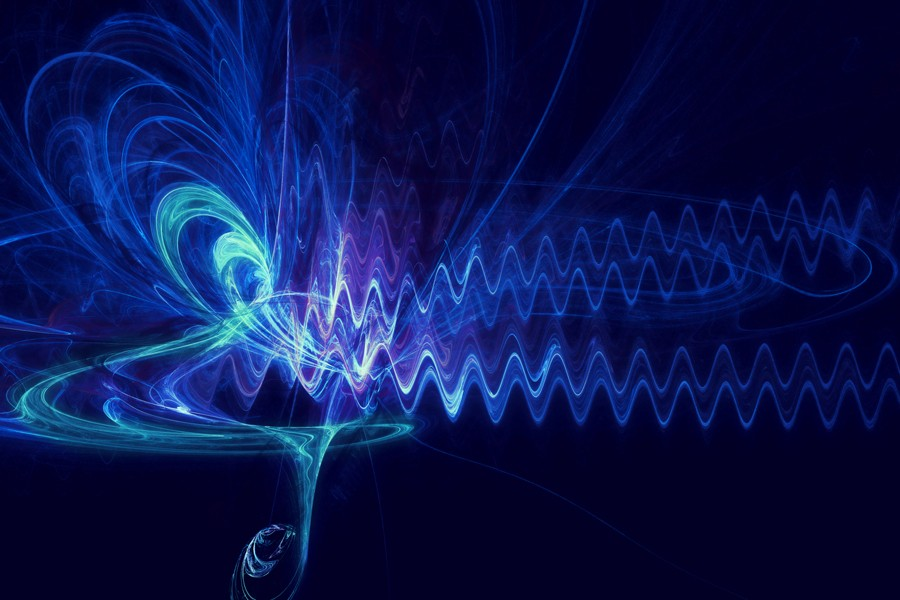
\includegraphics[width=0.65\textwidth]{timbre.jpg}
\end{figure}



\begin{minipage}{0.4\textwidth}
\begin{flushleft} \large
\emph{Author:}\\
Hannah \textsc{Shahba} 
\end{flushleft}
\begin{flushleft} \large
\emph{Author:}\\
Matt \textsc{Erickson} 
\end{flushleft}
\begin{flushleft} \large
\emph{Author:}\\
Liam \textsc{Nestelroad} 
\end{flushleft}
\end{minipage}
~
\begin{minipage}{0.4\textwidth}
\begin{flushright} \large
\emph{Professor:} \\
Dr. \textsc{Bhat} 
\end{flushright}
\begin{flushright} \large
\emph{Professor:} \\
Dr. \textsc{Segur} 
\end{flushright}
\end{minipage}\\[1cm]

{\large December 6, 2019}\\[2cm] 
 
\vfill

\end{titlepage}

\newpage
\renewcommand\contentsname{Table of Contents}
\doublespacing
\tableofcontents
\singlespacing
\addtocontents{toc}{~\hfill\textbf{Page}\par}
\newpage

\maketitle
\begin{abstract}


    
\end{abstract}

\newpage




\section{Abstract}

\section{1D Propagation}

\section{2D Propagation}
    
\section{3D Propagation}

\section{$n$-D Propagation}

\section{Conclusion}

\section{Acknowledgements}

    \begin{thebibliography}{}

    \bibitem{baker} Baker, N. 1966,
        in Stellar Evolution,
        ed.\ R. F. Stein \& A. G. W. Cameron
        (Plenum, New York) 333

    \bibitem{balluch} Balluch, M. 1988,
        A\&A, 200, 58

    \end{thebibliography}

\newpage
\end{document}


% \section*{Abstract}
 
% \section{1-D Propagation}

% \subsection{Example of mathematical formulas}

%    \begin{eqnarray}
%       \sigma_0 & = & \frac{\pi}{\sqrt{8}}
%                      \frac{1}{ \tau_{\mathrm{ff}}} \\
%       K        & = & \frac{\sqrt{32}}{\pi} \frac{1}{\delta}
%                         \frac{ \tau_{\mathrm{ff}} }
%                              { \tau_{\mathrm{co}} }\,;
%    \end{eqnarray}
 
% \noindent
    
%    \begin{equation}
%       \tau_{\mathrm{co}} = \frac{E_{\mathrm{th}}}{L_{r0}} \,,
%    \end{equation}


%    \begin{equation}
%       \tau_{\mathrm{ff}} =
%          \sqrt{ 
% 	 	\frac{3 \pi}{32 G} \frac{4\pi r_0^3}{3 M_{\mathrm{r}}}
% 	 }\,,
%    \end{equation}


%    \begin{displaymath}
%       \nabla_{\mathrm{ad}} = \left( \frac{ \partial \ln T}
%                              { \partial\ln P} \right)_{S} \, , \;
%       \chi^{}_T       = \left( \frac{ \partial \ln P}
%                              { \partial\ln T} \right)_{\rho} \, , \;
%       \kappa^{}_{T}   = \left( \frac{ \partial \ln \kappa}
%                              { \partial\ln T} \right)_{T}
%    \end{displaymath}

%    \begin{eqnarray}
%       \frac{\pi^2}{8} \frac{1}{\tau_{\mathrm{ff}}^2}
%                 ( 3 \Gamma_1 - 4 )
%          & > & 0 \label{ZSDynSta} \\
%       \frac{\pi^2}{\tau_{\mathrm{co}}
%                    \tau_{\mathrm{ff}}^2}
%                    \Gamma_1 \nabla_{\mathrm{ad}}
%                    \left[ \frac{ 1- 3/4 \chi^{}_\rho }{ \chi^{}_T }
%                           ( \kappa^{}_T - 4 )
%                         + \kappa^{}_P + 1
%                    \right]
%         & > & 0 \label{ZSSecSta} \\
%      \frac{\pi^2}{4} \frac{3}{\tau_{ \mathrm{co} }
%                               \tau_{ \mathrm{ff} }^2
%                              }
%          \Gamma_1^2 \, \nabla_{\mathrm{ad}} \left[
%                                    4 \nabla_{\mathrm{ad}}
%                                    - ( \nabla_{\mathrm{ad}} \kappa^{}_T
%                                      + \kappa^{}_P
%                                      )
%                                    - \frac{4}{3 \Gamma_1}
%                                 \right]
%         & > & 0   \label{ZSVibSta}
%    \end{eqnarray}

% \section{2-D Sound Propagations}

% \begin{table}[htb]
%       \caption[]{Example of table caption: opacity sources.}
%          \label{KapSou}
%      $$ 
%          \begin{array}{p{0.7\linewidth}l}
%             \hline
%             \noalign{\smallskip}
%             Source      &  T / {[\mathrm{K}]} \\
%             \noalign{\smallskip}
%             \hline
%             \noalign{\smallskip}
%             Yorke 1979, Yorke 1980a & \leq 1700           \\
%             Kr\"ugel 1971           & 1700 \leq T \leq 5000 \\
%             Cox \& Stewart 1969     & 5000 \leq             \\
%             \noalign{\smallskip}
%             \hline
%          \end{array}
%      $$ 
% \end{table}

% \section{n-D Sound Propagation}

% \section{Conclusions}



% \end{document}

